\documentclass{paper}
\usepackage{tikz}
\usetikzlibrary{shapes.geometric, arrows.meta, positioning}
\usepackage{geometry}
\usepackage{amsmath}
\usepackage{graphicx}
\usepackage{fancyhdr}
\usepackage{hyperref}

\hypersetup{
    colorlinks=true,
    linkcolor=blue,
    filecolor=magenta,      
    urlcolor=cyan,
}

\author{Balaji Karedla, Harith S, Sandeep Reddy Nallamilli}
\title{CS 791 - Assignment 1 Report}
\date{\today}

\begin{document}

\pagestyle{fancy}
\fancyhead{}
\fancyhead[L]{CS 791 - Assignment 1 Report}
\fancyhead[R]{\thepage}
\pagenumbering{roman}

\maketitle

\tableofcontents

\pagebreak

\pagenumbering{arabic}
\section{Factorial Hidden Markov Model (FHMM)}

An FHMM is an extension of the standard Hidden Markov Model (HMM) that allows for multiple independent hidden state sequences to influence the observed data.

The problem of interest is to infer the marginals of the hidden states, and the most probable sequence of hidden states, given a sequence of observations in a Factorial Hidden Markov Model (FHMM).

The problem involved making a junction tree out of the FHMM by triangulating it and then using the message passing algorithm to infer the marginals of the hidden states and the most probable sequence of hidden states given a sequence of observations.

\vspace{1cm}
\begin{center}
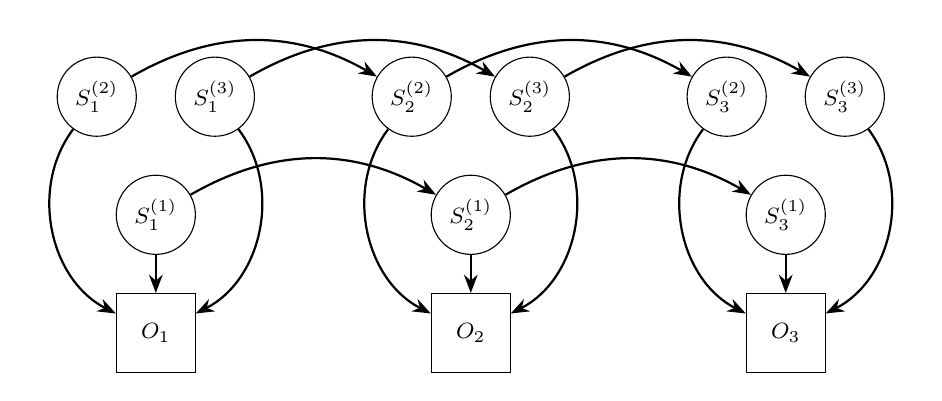
\begin{tikzpicture}[
    ->, >=Stealth, auto, node distance=3cm,
    state/.style={circle, draw, minimum size=0.8cm, font=\footnotesize},
    obs/.style={rectangle, draw, minimum size=1cm, font=\footnotesize},
    every edge/.style={draw, thick}
]

% Hidden states for Factor 1 (bottom of inverted triangle)
\node[state] (S1_1) at (0, 4) {$S_1^{(1)}$};
\node[state] (S1_2) at (4, 4) {$S_2^{(1)}$};
\node[state] (S1_3) at (8, 4) {$S_3^{(1)}$};

% Hidden states for Factor 2 (top-left of inverted triangle)
\node[state] (S2_1) at (-0.75, 5.5) {$S_1^{(2)}$};
\node[state] (S2_2) at (3.25, 5.5) {$S_2^{(2)}$};
\node[state] (S2_3) at (7.25, 5.5) {$S_3^{(2)}$};

% Hidden states for Factor 3 (top-right of inverted triangle)
\node[state] (S3_1) at (0.75, 5.5) {$S_1^{(3)}$};
\node[state] (S3_2) at (4.75, 5.5) {$S_2^{(3)}$};
\node[state] (S3_3) at (8.75, 5.5) {$S_3^{(3)}$};

% Observations (below the inverted triangle)
\node[obs] (O1) at (0, 2.5) {$O_1$};
\node[obs] (O2) at (4, 2.5) {$O_2$};
\node[obs] (O3) at (8, 2.5) {$O_3$};

% Transition edges for Factor 1 (more bent)
\path (S1_1) edge[bend left=30] (S1_2);
\path (S1_2) edge[bend left=30] (S1_3);

% Transition edges for Factor 2 (more bent)
\path (S2_1) edge[bend left=30] (S2_2);
\path (S2_2) edge[bend left=30] (S2_3);

% Transition edges for Factor 3 (more bent)
\path (S3_1) edge[bend left=30] (S3_2);
\path (S3_2) edge[bend left=30] (S3_3);

% Observation edges for t=1 (more bent)
\path (S1_1) edge (O1);
\path (S2_1) edge[bend right=50] (O1);
\path (S3_1) edge[bend left=50] (O1);

% Observation edges for t=2 (more bent)
\path (S1_2) edge (O2);
\path (S2_2) edge[bend right=50] (O2);
\path (S3_2) edge[bend left=50] (O2);

% Observation edges for t=3 (more bent)
\path (S1_3) edge (O3);
\path (S2_3) edge[bend right=50] (O3);
\path (S3_3) edge[bend left=50] (O3);

\end{tikzpicture}
\end{center}

The moralized graph looks like

\begin{center}
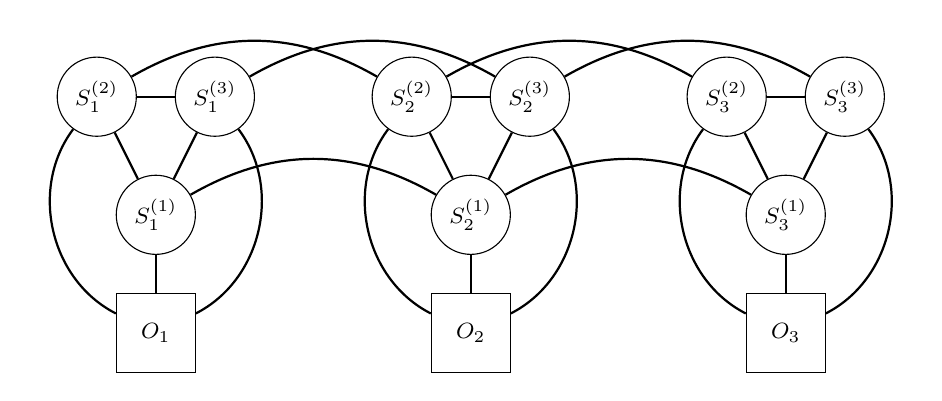
\begin{tikzpicture}[
    auto, node distance=3cm,
    state/.style={circle, draw, minimum size=0.8cm, font=\footnotesize},
    obs/.style={rectangle, draw, minimum size=1cm, font=\footnotesize},
    every edge/.style={draw, thick}
]

% Hidden states for Factor 1 (bottom of inverted triangle)
\node[state] (S1_1) at (0, 4) {$S_1^{(1)}$};
\node[state] (S1_2) at (4, 4) {$S_2^{(1)}$};
\node[state] (S1_3) at (8, 4) {$S_3^{(1)}$};

% Hidden states for Factor 2 (top-left of inverted triangle)
\node[state] (S2_1) at (-0.75, 5.5) {$S_1^{(2)}$};
\node[state] (S2_2) at (3.25, 5.5) {$S_2^{(2)}$};
\node[state] (S2_3) at (7.25, 5.5) {$S_3^{(2)}$};

% Hidden states for Factor 3 (top-right of inverted triangle)
\node[state] (S3_1) at (0.75, 5.5) {$S_1^{(3)}$};
\node[state] (S3_2) at (4.75, 5.5) {$S_2^{(3)}$};
\node[state] (S3_3) at (8.75, 5.5) {$S_3^{(3)}$};

% Observations (below the inverted triangle)
\node[obs] (O1) at (0, 2.5) {$O_1$};
\node[obs] (O2) at (4, 2.5) {$O_2$};
\node[obs] (O3) at (8, 2.5) {$O_3$};

% Transition edges for Factor 1 (undirected, curved)
\path (S1_1) edge[bend left=30] (S1_2);
\path (S1_2) edge[bend left=30] (S1_3);

\path (S1_1) edge (S2_1);
\path (S2_1) edge (S3_1);
\path (S3_1) edge (S1_1);

\path (S1_2) edge (S2_2);
\path (S2_2) edge (S3_2);
\path (S3_2) edge (S1_2);

\path (S1_3) edge (S2_3);
\path (S2_3) edge (S3_3);
\path (S3_3) edge (S1_3);

% Transition edges for Factor 2 (undirected, curved)
\path (S2_1) edge[bend left=30] (S2_2);
\path (S2_2) edge[bend left=30] (S2_3);

% Transition edges for Factor 3 (undirected, curved)
\path (S3_1) edge[bend left=30] (S3_2);
\path (S3_2) edge[bend left=30] (S3_3);

% Observation edges for t=1 (undirected, curved)
\path (S1_1) edge (O1);
\path (S2_1) edge[bend right=50] (O1);
\path (S3_1) edge[bend left=50] (O1);

% Observation edges for t=2 (undirected, curved)
\path (S1_2) edge (O2);
\path (S2_2) edge[bend right=50] (O2);
\path (S3_2) edge[bend left=50] (O2);

% Observation edges for t=3 (undirected, curved)
\path (S1_3) edge (O3);
\path (S2_3) edge[bend right=50] (O3);
\path (S3_3) edge[bend left=50] (O3);

\end{tikzpicture}
\end{center}

The junction tree made out of the cliques after triangulation is a chain as shown below:

\begin{center}
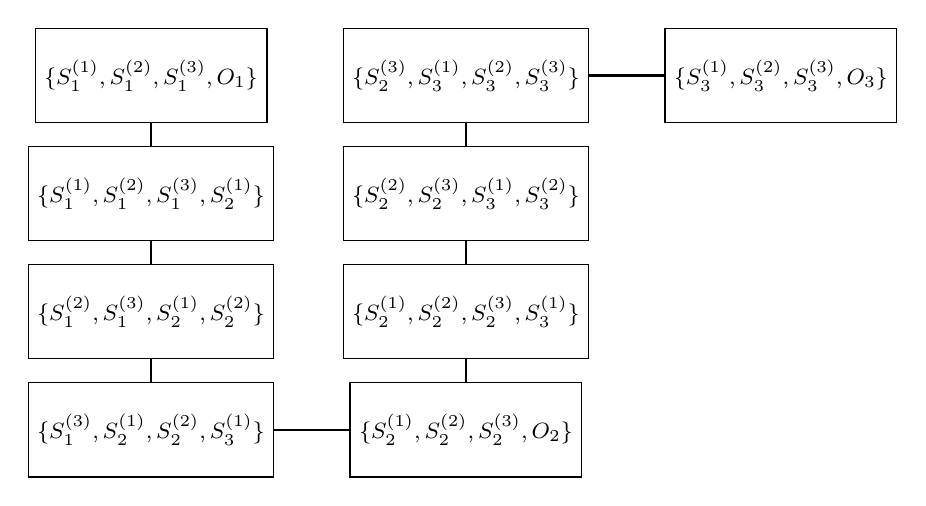
\begin{tikzpicture}[
    auto, node distance=4cm,
    clique/.style={rectangle, draw, minimum size=1.2cm, font=\footnotesize},
    every edge/.style={draw, thick}
]
% Cliques
\node[clique] (C1) at (0, 0) {$\{S_1^{(1)}, S_1^{(2)}, S_1^{(3)}, O_1\}$};
\node[clique] (C2) at (0, -1.5) {$\{S_1^{(1)}, S_1^{(2)}, S_1^{(3)}, S_2^{(1)}\}$};
\node[clique] (C3) at (0, -3) {$\{S_1^{(2)}, S_1^{(3)}, S_2^{(1)}, S_2^{(2)}\}$};
\node[clique] (C4) at (0, -4.5) {$\{S_1^{(3)}, S_2^{(1)}, S_2^{(2)}, S_3^{(1)}\}$};

\node[clique] (C5) at (4, -4.5) {$\{S_2^{(1)}, S_2^{(2)}, S_2^{(3)}, O_2\}$};
\node[clique] (C6) at (4, -3) {$\{S_2^{(1)}, S_2^{(2)}, S_2^{(3)}, S_3^{(1)}\}$};
\node[clique] (C7) at (4, -1.5) {$\{S_2^{(2)}, S_2^{(3)}, S_3^{(1)}, S_3^{(2)}\}$};
\node[clique] (C8) at (4, 0) {$\{S_2^{(3)}, S_3^{(1)}, S_3^{(2)}, S_3^{(3)}\}$};

\node[clique] (C9) at (8, 0) {$\{S_3^{(1)}, S_3^{(2)}, S_3^{(3)}, O_3\}$};
% Edges between cliques
\path (C1) edge (C2);
\path (C2) edge (C3);
\path (C3) edge (C4);
\path (C4) edge (C5);
\path (C5) edge (C6);
\path (C6) edge (C7);
\path (C7) edge (C8);
\path (C8) edge (C9);
\end{tikzpicture}
\end{center}

The message passing algorithm is now simple with just two passes, one from left to right and the other from right to left.

For including the prior of the observations, we merged the observations into the cliques by removing the observation nodes and considering the potentials over the cliques that include the observations.

For finding the z-value of the junction tree, the message passing algorithm runs over every clique for 

\newpage
\section{Loopy Belief Propagation}

Since exact inference is often computationally expensive, belief propagation (BP) is widely used as an approximate inference algorithm. The procedure starts by constructing a factor graph. We maintain beliefs for all variable nodes and factor nodes, and update them iteratively using a set of message-passing equations. On tree-structured graphs this yields exact marginals, while on graphs with loops, the same procedure (called loopy belief propagation) is only approximate.

The key idea is that if BP converges, it often converges to the correct marginal probabilities (exactly so in trees; approximately so in loopy graphs). However, because this is an iterative approximation algorithm, convergence is not guaranteed in general.

The order of message updates does not strictly matter, as long as all beliefs and messages are eventually updated. In my implementation, I update factor nodes first, then transition nodes, then send messages to variables, update variable beliefs, and finally send messages from variables back to factor and transition nodes. At each iteration, to avoid double counting, the contribution from the previous message that was already incorporated into a belief is divided out before incorporating new messages.

\begin{center}
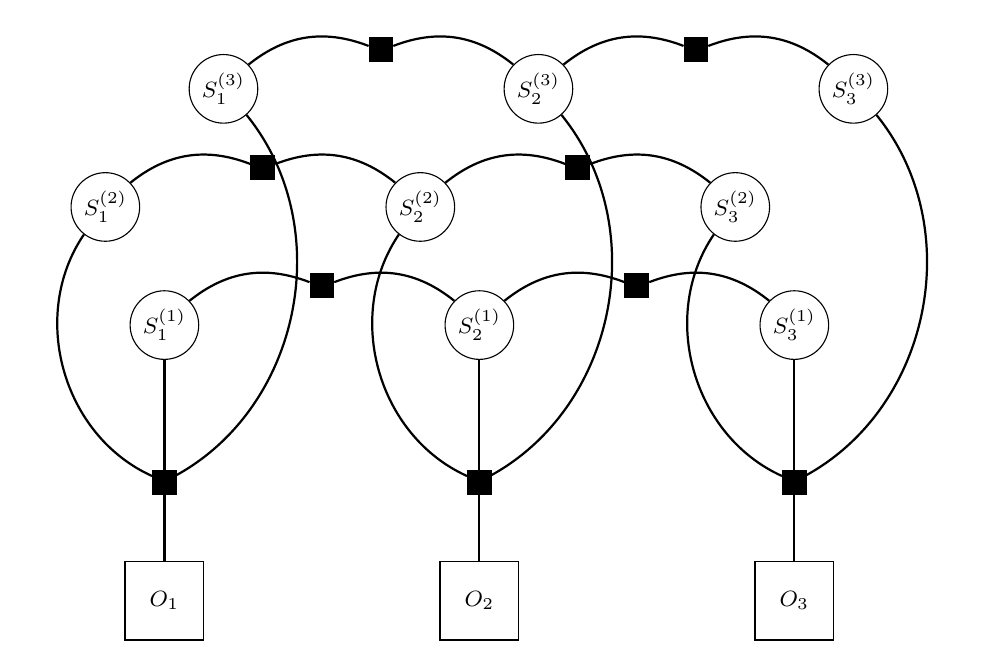
\begin{tikzpicture}[auto,
    var/.style={circle, draw, minimum size=0.8cm, font=\footnotesize, inner sep=2pt},
    factor/.style={rectangle, draw, fill=black, minimum size=0.3cm, font=\footnotesize, inner sep=0pt},
    obs/.style={rectangle, draw, minimum size=1cm, font=\footnotesize, inner sep=2pt},
    every edge/.style={draw, thick}
]

% Hidden state variables for Factor 1 (bottom row)
\node[var] (S1_1) at (0, 4) {$S_1^{(1)}$};
\node[var] (S1_2) at (4, 4) {$S_2^{(1)}$};
\node[var] (S1_3) at (8, 4) {$S_3^{(1)}$};

% Hidden state variables for Factor 2 (middle row, slightly offset)
\node[var] (S2_1) at (-0.75, 5.5) {$S_1^{(2)}$};
\node[var] (S2_2) at (3.25, 5.5) {$S_2^{(2)}$};
\node[var] (S2_3) at (7.25, 5.5) {$S_3^{(2)}$};

% Hidden state variables for Factor 3 (top row, slightly offset)
\node[var] (S3_1) at (0.75, 7) {$S_1^{(3)}$};
\node[var] (S3_2) at (4.75, 7) {$S_2^{(3)}$};
\node[var] (S3_3) at (8.75, 7) {$S_3^{(3)}$};

% Observation variables (below the hidden states)
\node[obs] (O1) at (0, 0.5) {$O_1$};
\node[obs] (O2) at (4, 0.5) {$O_2$};
\node[obs] (O3) at (8,0.5) {$O_3$};

% Factor nodes for transitions in Factor 1
\node[factor] (F1_T1) at (2, 4.5) {};
\node[factor] (F1_T2) at (6, 4.5) {};

% Factor nodes for transitions in Factor 2
\node[factor] (F2_T1) at (1.25, 6) {};
\node[factor] (F2_T2) at (5.25, 6) {};

% Factor nodes for transitions in Factor 3
\node[factor] (F3_T1) at (2.75, 7.5) {};
\node[factor] (F3_T2) at (6.75, 7.5) {};

% Factor nodes for observations
\node[factor] (F_O1) at (0, 2) {};
\node[factor] (F_O2) at (4, 2) {};
\node[factor] (F_O3) at (8, 2) {};

% Edges for Factor 1 transitions
\path (S1_1) edge[bend left=30] (F1_T1);
\path (F1_T1) edge[bend left=30] (S1_2);
\path (S1_2) edge[bend left=30] (F1_T2);
\path (F1_T2) edge[bend left=30] (S1_3);

% Edges for Factor 2 transitions
\path (S2_1) edge[bend left=30] (F2_T1);
\path (F2_T1) edge[bend left=30] (S2_2);
\path (S2_2) edge[bend left=30] (F2_T2);
\path (F2_T2) edge[bend left=30] (S2_3);

% Edges for Factor 3 transitions
\path (S3_1) edge[bend left=30] (F3_T1);
\path (F3_T1) edge[bend left=30] (S3_2);
\path (S3_2) edge[bend left=30] (F3_T2);
\path (F3_T2) edge[bend left=30] (S3_3);

% Edges for observation factors at t=1
\path (S1_1) edge (F_O1);
\path (S2_1) edge[bend right=50] (F_O1);
\path (S3_1) edge[bend left=50] (F_O1);
\path (F_O1) edge (O1);

% Edges for observation factors at t=2
\path (S1_2) edge (F_O2);
\path (S2_2) edge[bend right=50] (F_O2);
\path (S3_2) edge[bend left=50] (F_O2);
\path (F_O2) edge (O2);

% Edges for observation factors at t=3
\path (S1_3) edge (F_O3);
\path (S2_3) edge[bend right=50] (F_O3);
\path (S3_3) edge[bend left=50] (F_O3);
\path (F_O3) edge (O3);

\end{tikzpicture}
\end{center}

Let the number of states be \texttt{K}, number of states be \texttt{N}, number of factors be \texttt{M} and number of observations be \texttt{T}.

\begin{itemize}
    \item The function \texttt{updateFactorNodeBeliefs} has a time complexity of $O(TMK^M)$
    \item The function \texttt{updateTransitionNodeBeliefs} has a time complexity of $O(TMK^2)$
    \item The function \texttt{messageToSendFromFactor} has a time complexity of $O(MK^M)$
    \item The function \texttt{messageToSendFromTransition} has a time complexity of $O(K^2)$
    \item The resulting complexity of function \texttt{sendMessagesToVariables} is $O(TM^2K^M \texttt{+} TMK^2)$
    \item The function \texttt{updateVariableBeliefs} has a time complexity of $O(TMK)$
    \item The function \texttt{sendMessagesToFactorsNodes} has a time complexity of $O(TMK)$
    \item The function \texttt{sendMessagesToTransNodes} has a time complexity of $O(TMK)$
    \item Checking convergence has an order of $O(TMK)$
\end{itemize}
Therefore, the overall time complexity of the algorithm is $O(TM^2K^M \texttt{+} TMK^2)$ assuming O(1) iterations for convergence. 


\newpage
\section{Turbo Codes}

\subsection{Generating the Trellis}
The sequence of output bits is generated by computing the parity of the 
product between the generator polynomial and the contents of the shift register. 
If the shift register has length $k$, the encoder requires $2^{k-1}$ distinct states, 
since each new bit is obtained by appending the input bit to the register and 
then applying the parity operation. For every state and input pair, we compute both 
the next state of the register and the corresponding output parity bit. 
Using this information, we construct the trellis diagram over the full sequence 
of input bits.\\
Below is an example trellis with a shift register of length 3, generators 5 and 7, and a sequence of 4 bits. (Start state for any sequence is 00)

\begin{center}
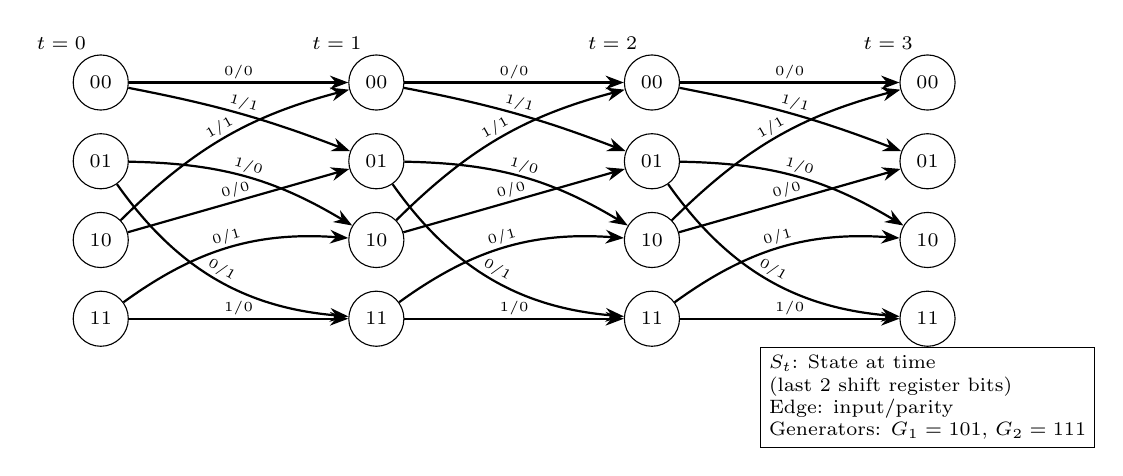
\begin{tikzpicture}[
    ->, >=Stealth, auto, node distance=3.5cm,
    state/.style={circle, draw, minimum size=0.7cm, font=\scriptsize, inner sep=1pt},
    edge label/.style={font=\tiny, midway, above, sloped, inner sep=1pt},
    every edge/.style={draw, thick}
]

% Time step labels
\node[font=\scriptsize] at (-0.5, 4.5) {$t=0$};
\node[font=\scriptsize] at (3, 4.5) {$t=1$};
\node[font=\scriptsize] at (6.5, 4.5) {$t=2$};
\node[font=\scriptsize] at (10, 4.5) {$t=3$};

% States at t=0
\node[state] (S0_0) at (0, 4) {$00$};
\node[state] (S1_0) at (0, 3) {$01$};
\node[state] (S2_0) at (0, 2) {$10$};
\node[state] (S3_0) at (0, 1) {$11$};

% States at t=1
\node[state] (S0_1) at (3.5, 4) {$00$};
\node[state] (S1_1) at (3.5, 3) {$01$};
\node[state] (S2_1) at (3.5, 2) {$10$};
\node[state] (S3_1) at (3.5, 1) {$11$};

% States at t=2
\node[state] (S0_2) at (7, 4) {$00$};
\node[state] (S1_2) at (7, 3) {$01$};
\node[state] (S2_2) at (7, 2) {$10$};
\node[state] (S3_2) at (7, 1) {$11$};

% States at t=3
\node[state] (S0_3) at (10.5, 4) {$00$};
\node[state] (S1_3) at (10.5, 3) {$01$};
\node[state] (S2_3) at (10.5, 2) {$10$};
\node[state] (S3_3) at (10.5, 1) {$11$};

% Transitions from t=0 to t=1
\path (S0_0) edge[edge label, above] node {$0/0$} (S0_1);
\path (S0_0) edge[edge label, bend left=5, above] node {$1/1$} (S1_1);
\path (S1_0) edge[edge label, bend right=25, above] node {$0/1$} (S3_1);
\path (S1_0) edge[edge label, bend left=15, above] node {$1/0$} (S2_1);
\path (S2_0) edge[edge label, above] node {$0/0$} (S1_1);
\path (S2_0) edge[edge label, bend left=15, above] node {$1/1$} (S0_1);
\path (S3_0) edge[edge label, bend left=20, above] node {$0/1$} (S2_1);
\path (S3_0) edge[edge label, above] node {$1/0$} (S3_1);

% Transitions from t=1 to t=2
\path (S0_1) edge[edge label, above] node {$0/0$} (S0_2);
\path (S0_1) edge[edge label, bend left=5, above] node {$1/1$} (S1_2);
\path (S1_1) edge[edge label, bend right=25, above] node {$0/1$} (S3_2);
\path (S1_1) edge[edge label, bend left=15, above] node {$1/0$} (S2_2);
\path (S2_1) edge[edge label, above] node {$0/0$} (S1_2);
\path (S2_1) edge[edge label, bend left=15, above] node {$1/1$} (S0_2);
\path (S3_1) edge[edge label, bend left=20, above] node {$0/1$} (S2_2);
\path (S3_1) edge[edge label, above] node {$1/0$} (S3_2);

% Transitions from t=2 to t=3
\path (S0_2) edge[edge label, above] node {$0/0$} (S0_3);
\path (S0_2) edge[edge label, bend left=5, above] node {$1/1$} (S1_3);
\path (S1_2) edge[edge label, bend right=25, above] node {$0/1$} (S3_3);
\path (S1_2) edge[edge label, bend left=15, above] node {$1/0$} (S2_3);
\path (S2_2) edge[edge label, above] node {$0/0$} (S1_3);
\path (S2_2) edge[edge label, bend left=15, above] node {$1/1$} (S0_3);
\path (S3_2) edge[edge label, bend left=20, above] node {$0/1$} (S2_3);
\path (S3_2) edge[edge label, above] node {$1/0$} (S3_3);

% Legend
\node[font=\scriptsize, align=left, draw, inner sep=3pt] at (10.5, 0) {
    $S_t$: State at time \\ 
    (last 2 shift register bits) \\
    Edge: input/parity \\
    Generators: $G_1=101$, $G_2=111$
};

\end{tikzpicture}
\end{center}

\subsection{Viterbi}
The algorithm begins in state $0$ with an initial cost of $0$, while all other 
states are assigned an infinite cost. Here, the cost represents the negative 
log likelihood of the most probable sequence leading to a particular state. 
\\During the forward pass, the algorithm iterates over each time step 
(corresponding to one bit of the original sequence) and evaluates all possible 
states at that step. For every possible input bit, it computes the likelihood of 
observing both the systematic and parity bits. These likelihoods are converted 
to costs and added to the cumulative cost of reaching the current state. If this 
new path yields a lower cost than any previously recorded path to the next state, 
the cost is updated along with a backpointer to record the optimal predecessor. 
\\In the backtracking phase, the algorithm identifies the final state with the 
minimum cumulative cost (equivalently, the maximum likelihood). Starting from 
this state, it follows the backpointers in reverse through the trellis, thereby 
reconstructing the most probable sequence of input bits.

The time complexity of the algorithm is $O(T * S)$ where $T$ is the length of the original string or the number of timestamps and $S$ is the total number of states (in this case $2^{k - 1}$) where k is the length of the shift register.

\subsection{BCJL and Turbo Codes}
In turbo decoding, a posteriori probabilities (APPs) are estimated with the BCJR algorithm, starting from uniform priors ($P(b=0)=P(b=1)=\tfrac{1}{2}$). For each received sequence, BCJR computes log-likelihood ratios (LLRs):
\[
    LLR_i = \log \frac{P(u_i=1 \mid \mathbf{y})}{P(u_i=0 \mid \mathbf{y})},
\]
where $u_i$ is the transmitted bit and $\mathbf{y}$ the channel output.
\\Each decoder then forms \emph{extrinsic information} by removing the prior 
contribution:
\[
    LLR^{\text{extrinsic}}_i = LLR_i - LLR^{\text{prior}}_i,
\] 
\[
    LLR^{\text{prior}}_i = \log \frac{P(u_i=1)}{P(u_i=0)}.
\]
These extrinsic values are interleaved and passed to the other decoder as new priors. Iterating this exchange gradually refines the APPs.
\\Convergence is monitored via the maximum LLR change,
\[
    \Delta = \max_i \left| LLR^{(t)}_i - LLR^{(t-1)}_i \right|,
\]
stopping early if $\Delta$ falls below a threshold, or otherwise after a fixed maximum number of iterations.

\subsection{Results}
% Run the code multiple times, for sizes 1000, 2000, 5000, 10000
% Write down the average BER (bit error rate)
We compared the decoding performance of three algorithms: the Viterbi decoder, 
the BCJR (MAP) decoder, and the Turbo decoder. The cumulative average BERs across 
all experiments are summarised below (and in results.txt):

\begin{itemize}
    \item Viterbi decoder: \textbf{3.90\%}
    \item BCJR decoder: \textbf{3.61\%}
    \item Turbo decoder: \textbf{0.0067\%}
\end{itemize}
In terms of BER, BCJL performs slightly better than Viterbi on average. This might be because BCJL gives the probability for each bit individually. The average length of a matched string is better in Viterbi, probably because Viterbi outputs the most probable string.
\\Since the turbo code always has almost zero errors, applying Viterbi on the final APP helps but does not improve the BER to any significant degree.

\newpage
\section{Contributions}
\begin{itemize}
    \item \textbf{Message Passing on Factorial HMMs: } Balaji Karedla
    \item \textbf{Loopy Belief Propagation: } Harith S
    \item \textbf{Turbo Codes: } Sandeep Reddy Nallamilli
\end{itemize}

\section{LLM Usage}
\begin{itemize}
    \item \textbf{Message Passing on Factorial HMMs (Q1)}
    \begin{itemize}
        \item Just a bit of CoPilot auto-completion for the idea I had in mind
        \item Never used a prompt to generate code or copied code from LLMs explicitly
    \end{itemize}
    \item \textbf{Loopy Belief Propagation (Q2)}
    \begin{itemize}
        \item Initialising factor beliefs (partly, was debugged with LLMs)
        \item \texttt{assignmentToIndex} function
        \item \texttt{normalise} function
        \item Divide by 0 handling 
        \item Checking for convergence
    \end{itemize}
    \item \textbf{Turbo Codes (Q3)}
    \begin{itemize}
        \item Clarified some doubts in how the BCJR algorithm worked
        \item Debugging numerical overflow and underflow errors
        \item Creating the tikz diagram for the report
        \item Other latex formatting
    \end{itemize}
\end{itemize}
\end{document}
